% Presentación del proyecto final (5 min + preguntas), 01-10-2026.
% Compilar con xelatex, dos veces:  xelatex presentacion.tex
% La figura de los decaimientos sale de presentacion/figura_decaimiento.py.
% Cada número sale de DECISIONES.md; la etiqueta va en azul claro al lado.
\documentclass[aspectratio=169,10pt]{beamer}
\usetheme[progressbar=frametitle,numbering=fraction,sectionpage=none,block=fill]{metropolis}
\usepackage{fontspec}
\setsansfont{Inter}[Scale=0.92]
\usefonttheme[onlymath]{serif}
\usepackage[spanish,es-noquoting]{babel}
\usepackage{tikz}
\usetikzlibrary{patterns,arrows.meta,positioning,calc}
\usepackage{booktabs}
\usepackage{amssymb}
\usepackage{bm}
\usepackage{appendixnumberbeamer}   % el total no cuenta el respaldo
\graphicspath{{figuras/}}

% ---------- paleta: dos azules y blanco ----------
\definecolor{azul}{HTML}{1F4E79}
\definecolor{azulc}{HTML}{7FA7CF}
\definecolor{azulf}{HTML}{EAF1F8}
\definecolor{tinta}{HTML}{1E2A38}
\setbeamercolor{normal text}{fg=tinta,bg=white}
\setbeamercolor{background canvas}{bg=white}
\setbeamercolor{frametitle}{bg=azul,fg=white}
\setbeamercolor{progress bar}{fg=azulc,bg=azul}
\setbeamercolor{title separator}{fg=azulc}
\setbeamercolor{alerted text}{fg=azul}
\setbeamerfont{alerted text}{series=\bfseries}
\setbeamerfont{frametitle}{size=\large,series=\bfseries}
\setbeamertemplate{itemize item}{\color{azul}\textbullet}
\setbeamertemplate{enumerate item}{\color{azul}\bfseries\insertenumlabel.}

\newcommand{\etq}[1]{{\color{azulc}\scriptsize[#1]}}
\newcommand{\repo}{github.com/Lucia-Maz/free-slip-boundary-conditions-fourier-continuation}

% un intervalo con topes, en una recta: x1, x2, y, color, media altura del tope
\newcommand{\intervalo}[5]{%
  \draw[line width=1.4pt,#4] ({#1},{#3}) -- ({#2},{#3});
  \draw[line width=1.4pt,#4] ({#1},{#3-#5}) -- ({#1},{#3+#5});
  \draw[line width=1.4pt,#4] ({#2},{#3-#5}) -- ({#2},{#3+#5});}

% eje cortado de la slide de validación: tramo A 0,058-0,090 y tramo B 0,270-0,294, 60 cm por s^-1
\newcommand{\ejeA}[1]{{1.55+60*(#1-0.058)}}
\newcommand{\ejeB}[1]{{3.77+60*(#1-0.270)}}

% ---------- portada y cierre: el mismo diseño ----------
\newcommand{\portada}[2]{%
\begin{frame}[plain]
\begin{tikzpicture}[remember picture,overlay]
  \fill[azul] (current page.north west) rectangle ([yshift=-0.35cm]current page.north east);
  \node[anchor=south,font=\footnotesize\ttfamily,text=azul] (gh) at ([yshift=0.55cm]current page.south) {\repo};
  \node[anchor=south,font=\small,text=azul] at ([yshift=4pt]gh.north) {Ondas Gravitacionales e Investigación Asistida por IA \,--\, 1 de octubre de 2026};
\end{tikzpicture}
\vspace*{0.1cm}
{\fontsize{24}{28}\selectfont\bfseries\color{azul} #1}\par
\vspace{6pt}
\if\relax\detokenize{#2}\relax\else{\large\color{tinta} #2}\par\fi
\vspace{10pt}
{\color{azulc}\rule{\textwidth}{0.6pt}}\par
\vspace{8pt}
{\large\bfseries Lucía Mazaira}\par
\vspace{2pt}
{\normalsize INFINA, CONICET--UBA}\par
\end{frame}}

% ---------- un panel de la capa: #1 = rigida | libre ----------
\newcommand{\capa}[1]{%
\begin{tikzpicture}[x=1cm,y=1cm]
  \def\H{2.0}\def\W{3.4}\def\A{1.7}
  \fill[azulf] (0,0) rectangle (\W,\H);
  \fill[pattern=north east lines,pattern color=azulc] (0,-0.28) rectangle (\W,0);
  \draw[azul,line width=1.1pt] (0,0) -- (\W,0);
  \def\tipo{#1}\def\rig{rigida}
  \ifx\tipo\rig
    \fill[pattern=north east lines,pattern color=azulc] (0,\H) rectangle (\W,\H+0.28);
    \draw[azul,line width=1.1pt] (0,\H) -- (\W,\H);
    \def\f##1{sin(180*##1/\H)}
    \colorlet{perfil}{azulc}
  \else
    \draw[azul,line width=1.4pt] plot[domain=0:\W,samples=60] (\x,{\H+0.06*sin(\x*260)});
    \node[azulc,font=\scriptsize] at (\W/2,\H+0.3) {aire};
    \def\f##1{sin(90*##1/\H)}
    \colorlet{perfil}{azul}
  \fi
  \draw[{Stealth[length=3pt]}-{Stealth[length=3pt]},tinta,line width=0.6pt] (\W-0.3,0.03) -- (\W-0.3,\H-0.03)
       node[midway,left,font=\footnotesize,text=tinta] {$h$};
  \draw[azulc,line width=0.5pt] (0.35,0) -- (0.35,\H);
  \draw[perfil,line width=1.5pt] plot[variable=\z,domain=0:\H,samples=40] ({0.35+\A*\f{\z}},{\z});
  \foreach \z in {0.4,0.8,1.2,1.6,1.98}
    \draw[-{Stealth[length=3.5pt]},perfil,line width=0.8pt] (0.35,\z) -- ({0.35+\A*\f{\z}},\z);
\end{tikzpicture}}

% ---------- la escalera de las tres condiciones ----------
\newcommand{\escalera}{%
\begin{tikzpicture}[
  nivel/.style={draw=azul,line width=0.8pt,rounded corners=4pt,fill=white,
                minimum height=1.3cm,text width=4.0cm,align=center,inner sep=3pt,font=\footnotesize},
  flecha/.style={-{Stealth[length=5pt]},line width=1.1pt,color=azulc},
  estado/.style={rounded corners=3pt,font=\scriptsize\bfseries,text=white,fill=azul,inner sep=2.5pt}]
  \node[nivel] (n1) {{\bfseries\color{azul}1 · free-slip plano}\\[1pt]
     {\color{azul!70}superficie fija en $z=h$}\\[3pt] \mbox{$w=0$}};
  \node[nivel,right=0.4cm of n1] (n2) {{\bfseries\color{azul}2 · deformable, lineal}\\[1pt]
     {\color{azul!70}orden 1: sólo el primer término}\\[3pt] \mbox{$\partial_t\eta=w$}};
  \node[nivel,right=0.4cm of n2] (n3) {{\bfseries\color{azul}3 · deformable, orden $N$}\\[1pt]
     {\color{azul!70}por ejemplo $N=2$}\\[3pt]
     \mbox{$\partial_t\eta=w+{\color{azul}\bm{\eta\,\partial_z w-\mathbf u_h\!\cdot\!\nabla\eta}}$}};
  \draw[flecha] (n1) -- (n2);
  \draw[flecha] (n2) -- (n3);
  \node[estado,anchor=north] at ([yshift=-3pt]n1.south) {verificado · 6/6};
  \node[estado,anchor=north] at ([yshift=-3pt]n2.south) {verificado · 8/8};
  \node[estado,anchor=north,fill=azulc] at ([yshift=-3pt]n3.south) {funciona, con límites · 4/10};
\end{tikzpicture}}

\begin{document}

\portada{La superficie libre en SPECTER}{Implementar la condición de contorno de una capa delgada:\\
de \emph{free-slip} plano a una superficie deformable de orden $N$}

%======================================================================
\begin{frame}[t]{Objetivo: la condición de contorno que le faltaba a SPECTER}
\vspace{2pt}
\begin{columns}[T,onlytextwidth]
\column{0.52\textwidth}
\centering
\begin{tabular}{@{}c@{\hspace{0.4cm}}c@{}}
{\small\bfseries\color{azulc} tapa rígida} & {\small\bfseries\color{azul} superficie libre}\\[4pt]
\capa{rigida} & \capa{libre}\\[2pt]
{\footnotesize $u\propto\sin(\pi z/h)$} & {\footnotesize $u\propto\sin(\pi z/2h)$}\\[3pt]
{\color{azulc}$\alpha=\dfrac{\nu\pi^2}{h^2}$} & {\color{azul}$\alpha=\dfrac{\nu\pi^2}{4h^2}$}\\
\end{tabular}

\vspace{6pt}
{\footnotesize fondo no-deslizante en ambos casos}

\column{0.45\textwidth}
\small
\begin{itemize}\setlength{\itemsep}{5pt}
\item \textbf{Mi experimento:} estudio el \textbf{decaimiento} de flujos en capas delgadas (6 mm), con fondo sólido y superficie libre. Mido la velocidad en la superficie con PIV.
\item Al dejar de forzarlo, el flujo decae por \textbf{fricción con el fondo}, $-\alpha\,\mathbf u$. Lo que hay arriba cambia $\alpha$ \textbf{un factor 4}.
\item Para simularlos con sus bordes uso \textbf{SPECTER}, que sólo tenía no-deslizamiento: $\alpha$ se ajustaba a mano.
\item \textbf{Objetivo:} implementar la superficie libre. La motiva mi experimento; sirve para cualquier flujo con el tope abierto.
\end{itemize}
\end{columns}
\end{frame}

%======================================================================
\begin{frame}[t]{Resultado: tres niveles de la misma condición}
\vspace{2pt}
\centering\escalera

\vspace{12pt}
\raggedright\small
La superficie está en $z=h+\eta$, pero la malla termina en $z=h$. Cada condición se traslada con Taylor:
\[
f(h+\eta)=\underbrace{f(h)}_{\text{nivel 2}}\;+\;\underbrace{\eta\,\partial_z f(h)+\tfrac12\,\eta^2\,\partial_z^2 f(h)+\dots}_{\text{nivel 3: hasta orden }N}
\]
\vspace{-4pt}
\begin{itemize}\setlength{\itemsep}{3pt}
\item \textbf{Nivel 1:} la superficie no se mueve ($\eta=0$). Sólo se anula la tensión tangencial.
\item \textbf{Nivel 2:} $\eta$ es un campo propio, pero todo se evalúa en $z=h$ y se queda lo \textbf{lineal} en la amplitud.
\item \textbf{Nivel 3:} se suman los términos $\eta\,\partial_z(\cdot)$ y los de la pendiente $\nabla\eta$, hasta $N=2$ o 3. Lo mismo con las tensiones.
\end{itemize}
\end{frame}

%======================================================================
\begin{frame}[t]{Resultado: la superficie, a la escala de mi celda}
\centering
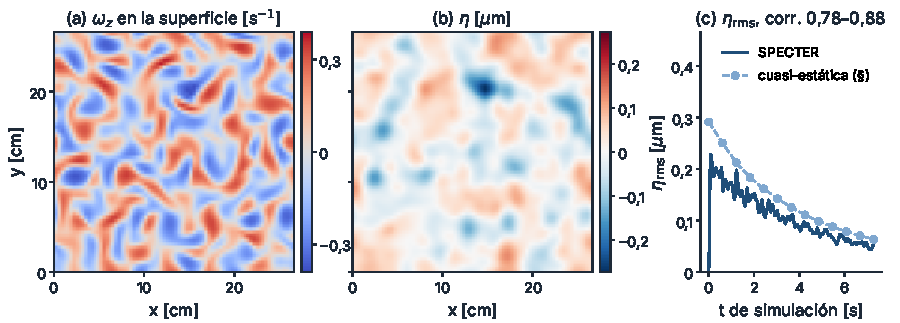
\includegraphics[width=0.94\textwidth]{f_fs6_superficie_pres.pdf}

\vspace{4pt}
\raggedright\small
\begin{itemize}\setlength{\itemsep}{3pt}
\item Nivel 3 con $N=2$, $g$ y tensión superficial físicas; condición inicial: el espectro medido por PIV.
\item Mismo instante, $t=7{,}3$ s. $\eta$ sigue a la presión: la superficie \textbf{se hunde donde la presión baja}, en los vórtices. Pozos de hasta $-0{,}27\,\mu$m, lomas de sólo $+0{,}13$.
\item $\eta_{\rm rms}\le0{,}23\,\mu$m sobre 6 mm: \textbf{free-slip plano era buena aproximación}, ahora calculado. \etq{V-23}
\end{itemize}
\end{frame}

%======================================================================
\begin{frame}[t]{Validación: ¿se parece a lo que mido?}
\begin{columns}[T,onlytextwidth]
\column{0.58\textwidth}
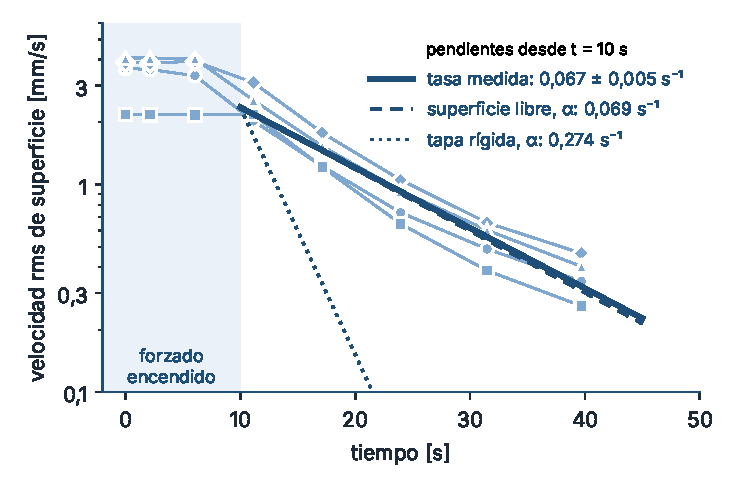
\includegraphics[width=0.94\textwidth]{decaimiento_azul.pdf}

\vspace{-2pt}
{\footnotesize Cuatro decaimientos medidos con PIV; ajuste para $t>10$ s. \etq{V-13}}

\vspace{6pt}
{\color{azulc}\rule{\linewidth}{0.4pt}}\\[3pt]
\footnotesize\textbf{En el código:} pruebas escritas antes de implementar, que pueden fallar: 6/6 · 6/6 · 8/8 · 4/10.

\column{0.39\textwidth}
\vspace{2pt}
\textbf{La tasa medida, contra la calculada}\\[10pt]
% eje cortado, misma escala en los dos tramos: 60 cm por s^-1
% tramo A: 0,058-0,090 en x = 1,55 ... 3,47; tramo B: 0,270-0,294 en x = 3,77 ... 5,21
% predicciones: alpha + nu k^2 con k = 59-130 m^-1 (las imprime presentacion/figura_decaimiento.py, [P-02])
\begin{tikzpicture}[x=1cm,y=1cm]
  % ejes
  \draw[azulc,line width=0.6pt] (1.55,0) -- (3.47,0);
  \draw[azulc,line width=0.6pt] (3.77,0) -- (5.21,0);
  \foreach \x in {3.47,3.77} \draw[azulc,line width=0.6pt] ({\x-0.06},-0.1) -- ({\x+0.06},0.1);
  \foreach \v/\t in {0.06/0{,}06,0.07/0{,}07,0.08/0{,}08,0.09/{}}
    \draw[azulc] (\ejeA{\v},0.06) -- (\ejeA{\v},-0.06) node[below,font=\scriptsize,text=tinta] {\t};
  \foreach \v/\t in {0.27/{},0.28/0{,}28,0.29/0{,}29}
    \draw[azulc] (\ejeB{\v},0.06) -- (\ejeB{\v},-0.06) node[below,font=\scriptsize,text=tinta] {\t};
  \node[azul,font=\scriptsize] at (3.38,-0.6) {tasa de decaimiento [s$^{-1}$]};
  % filas
  \foreach \y/\t in {1.4/tapa rígida,0.92/superficie libre,0.44/medido}
    \node[azul,font=\scriptsize,anchor=east] at (1.45,\y) {\t};
  \intervalo{\ejeB{0.2776}}{\ejeB{0.2910}}{1.4}{azul}{0.09}
  \intervalo{\ejeA{0.0720}}{\ejeA{0.0854}}{0.92}{azul}{0.09}
  \intervalo{\ejeA{0.06199}}{\ejeA{0.07175}}{0.44}{azul}{0.09}
  \fill[azul] (\ejeA{0.06687},0.44) circle (2.4pt);
\end{tikzpicture}

\vspace{8pt}
\small
Tapa rígida: \textbf{cuatro veces más rápido}. Superficie libre: cerca de lo medido.

\vspace{5pt}
{\scriptsize\color{azul!60}Las predicciones suman a $\alpha$ la disipación horizontal $\nu k^2$, con el $k$ del flujo. Salvedad abierta: la tasa medida queda 7--22\,\% debajo. \etq{P-02}}
\end{columns}
\end{frame}

%======================================================================
\begin{frame}[t]{Aprendizaje: ¿la prueba podía fallar?}
\begin{columns}[T,onlytextwidth]
\column{0.58\textwidth}
\small
\textbf{Lo que me pasó} \etq{H-13}
\begin{enumerate}\setlength{\itemsep}{4pt}
\item Para medir un efecto nuevo, reusé el caso de una prueba que ya pasaba (\textbf{6/6}).
\item Corrí dos resoluciones distintas, y dieron \textbf{idénticas, hasta la última cifra}.
\item Eso sólo pasa si lo medido es \alert{exactamente cero}: el caso anulaba justo el término que quería medir.
      La prueba pasaba \textbf{por default}.
\end{enumerate}

\vspace{6pt}
\textbf{Qué cambié}
\begin{itemize}\setlength{\itemsep}{4pt}
\item Cada prueba incluye ahora \textbf{un caso que tiene que fallar}.
\item Dejo escrito \textbf{qué no verifica} cada prueba.
\end{itemize}

\column{0.38\textwidth}
\vspace{8pt}
\begin{tikzpicture}
  \node[fill=azul,text=white,rounded corners=6pt,text width=0.9\linewidth,
        inner sep=10pt,align=left,font=\small]
    {\hyphenpenalty=10000\exhyphenpenalty=10000 Ahora, cuando una prueba pasa, me pregunto:\\[8pt]
     {\color{azulf}\bfseries ¿podría haber fallado?}\\[3pt]
     {\color{azulf}es decir, ¿es falsable?}};
\end{tikzpicture}

\vspace{12pt}
{\footnotesize\color{azul!60} Con agentes me parece aún más importante: si quien escribe el código puede editar la prueba, que pase dice poco.}
\end{columns}
\end{frame}

%======================================================================
\portada{¡Gracias!}{}

%======================================================================
% ------------------------- RESPALDO (preguntas) -----------------------
\appendix
\setbeamertemplate{frame numbering}[none]   % el respaldo no va numerado

\begin{frame}[t]{Respaldo · por qué free-slip plano no tiene error de partición}
\small
SPECTER avanza un campo sin presión $\mathbf v^*$, le impone una condición y proyecta:
\[
\mathbf v=\mathbf v^*-\tfrac{\Delta t}{o}\nabla p,\qquad \partial_z p=\tfrac{o}{\Delta t}\,v^*_z\ \ \text{(Neumann, como un canal)}.
\]
Pedir tensión tangencial nula sobre el campo \emph{proyectado} da, sobre $\mathbf v^*$,
\[
\partial_z v^*_x = i k_x v^*_z,\quad \partial_z v^*_y = i k_y v^*_z
\quad\Longleftrightarrow\quad \omega^*_x=\omega^*_y=0\ \text{en la cara.}
\]
No aparece $\Delta t$, y como $\nabla\times\nabla p=0$, \ $\nabla\times\mathbf v^*=\nabla\times\mathbf v$ exactamente. \etq{D-24}
\begin{itemize}\setlength{\itemsep}{3pt}
\item \textbf{Predicción falsable:} el residuo no depende de $\Delta t$. Medido: $6{,}1\cdot10^{-12}$, y el cociente entre $\Delta t$ y $\Delta t/2$ da \textbf{1,00}.
\item El no-deslizamiento, en cambio, deja un deslizamiento que escala como $\Delta t^{4{,}004}$. \etq{V-15}
\item Con superficie deformable, $\partial_x w\neq0$ y la tensión deja de ser la vorticidad: la propiedad se pierde.
\end{itemize}
\end{frame}

\begin{frame}[t]{Respaldo · las pruebas, con sus números}
\small
Escritas antes del código, arrancan fallando, se congelan por hash y \textbf{no contienen la fórmula}: arman su propia referencia (diferencias finitas y extrapolación de Richardson).

\vspace{6pt}
\begin{tabular}{@{}l l r@{}}
\toprule
& lo que se mide & \\
\midrule
teoría & $\alpha=\nu\pi^2/4h^2$ y el factor 4 contra tapa rígida & 6/6\\
nivel 1 & tasa del modo lento: error $6{,}8\cdot10^{-10}$; cociente $4{,}000000015$ & 6/6\\
nivel 2 & $\eta(t)$ contra una referencia MAC: $1{,}2\cdot10^{-6}$; orden temporal 2,00 & 8/8\\
nivel 3 & orden $N$: el modelo es exacto a $10^{-14}$; $N=3$ tiene orden 3 en una onda no lineal & 4/10\\
\bottomrule
\end{tabular}

\vspace{8pt}
Cada una incluye un caso que tiene que fallar (en la Fase 5, cuatro modelos equivocados quedan a $250\times$ la tolerancia).
El verificador independiente es de otra familia de modelos que el que implementó. \etq{V-07, V-09, V-20, V-22}
\end{frame}

\begin{frame}[t]{Respaldo · el 4/10 del orden $N$: fallos que son hallazgos}
\small
La prueba se escribió antes, arrancó fallando (1/10) y \textbf{no se editó}. Ninguno de los seis fallos es un error de programación. \etq{V-21}
\begin{itemize}\setlength{\itemsep}{5pt}
\item \textbf{$N=2$ está mal planteado donde $\eta<0$}: admite una capa espuria de espesor $|\eta|$ que crece como $\nu/\eta^2$. El código aborta antes de llegar ahí. \etq{H-24}
\item \textbf{Con elevación uniforme, $N=2$ ya es $O(\eta^3)$}: el criterio de la prueba estaba mal a priori. \etq{H-25}
\item \textbf{La tercera derivada espectral en el borde} tiene un piso que limita a $N=3$. \etq{H-26}
\item El cierre fijado en el diseño era inestable en el tiempo; se reemplazó. \etq{H-23}
\end{itemize}
\vspace{4pt}
En la celda no aplica ningún límite: $\eta/\Delta z\sim10^{-3}$.
\end{frame}

\begin{frame}[t]{Respaldo · la salvedad del contraste}
\small
\begin{itemize}\setlength{\itemsep}{6pt}
\item Lo que se mide es una \textbf{tasa total}, $\lambda_{\rm medida}=0{,}067\pm0{,}005$ s$^{-1}$: incluye la fricción de fondo y la viscosidad horizontal. $\alpha$ es sólo la fricción, y coincide con la tasa en el límite $k\to0$.
\item Con el $k$ que el flujo tiene en la ventana del ajuste (59--130 m$^{-1}$), la tasa predicha es $\lambda=\alpha+\nu k^2=0{,}072$--$0{,}085$ s$^{-1}$: la medida queda \textbf{7--22\,\% abajo}. \etq{P-02}
\item \textbf{La no linealidad empuja al revés}: sube la fricción de fondo hasta un 26\,\% en $\delta=10$. \etq{V-16}
\item Ajustando la tasa medida anillo por anillo, $\lambda(k)=0{,}048+\nu k^2$: recupera $\nu$ sin imponerla, y el faltante queda en la ordenada. \etq{V-18}
\item Un fondo de movimiento con la forma de la red de imanes explica un 4--5\,\%. \etq{H-18}
\item Medio milímetro de error en $h$ mueve $\alpha$ un 17\,\%.
\end{itemize}
\end{frame}

\begin{frame}[t]{Respaldo · qué le hace la no linealidad a la fricción}
\centering
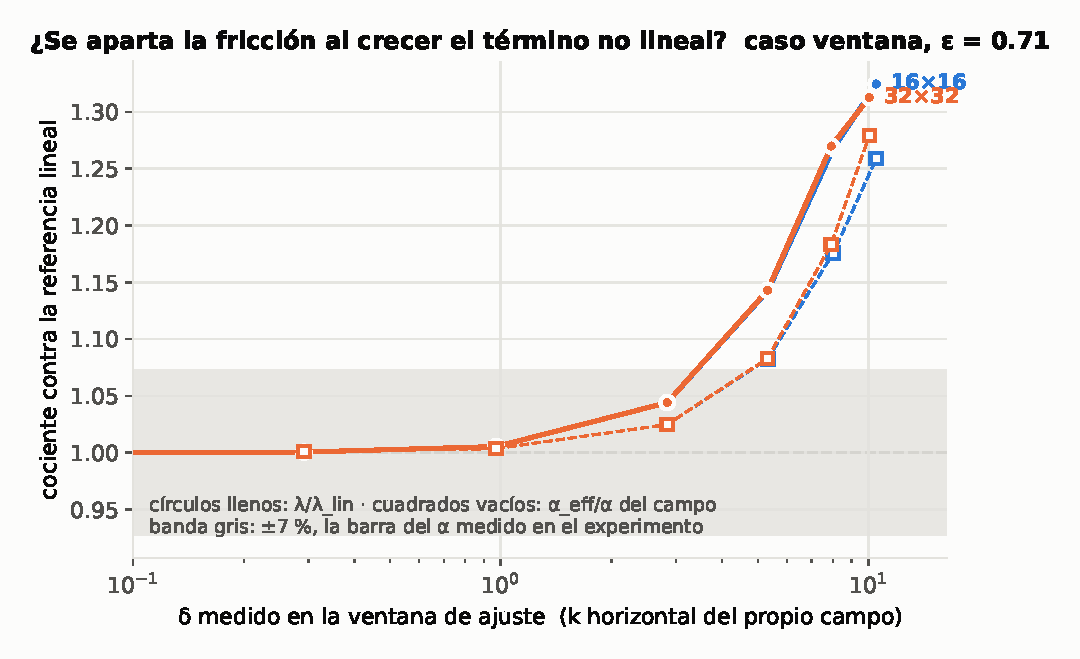
\includegraphics[width=0.48\textwidth]{f7_barrido_delta_ventana.pdf}\hfill
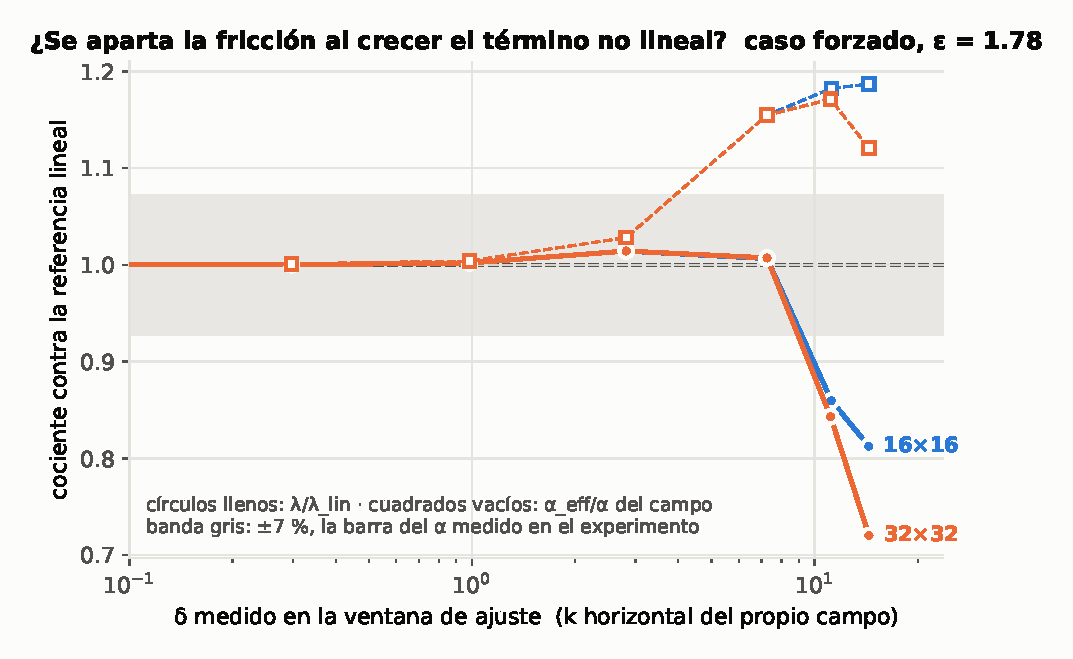
\includegraphics[width=0.48\textwidth]{f7_barrido_delta_forzado.pdf}

\vspace{4pt}
\small
Con $\delta=Ukh^2/\nu$, la fricción de fondo \textbf{sube}: $+2{,}5\%$ en $\delta=3$ y $+26\%$ en $\delta=10$.
Un PIV de superficie ve menos: la tasa de $u(h)$ queda entre $+3$ y $+12\%$ de la lineal. \etq{V-16, V-17}
\end{frame}

\end{document}
